\documentclass[9pt]{extarticle}

\usepackage[a4paper, total={6in, 8in}]{geometry}
\usepackage[utf8]{inputenc}
\usepackage{newunicodechar}
\usepackage{tikz}
\usepackage{verbatim}
\usetikzlibrary{trees}

\newunicodechar{⊥}{$\bot$}
\DeclareUnicodeCharacter{22A5}{$\bot$}
\DeclareUnicodeCharacter{03BB}{$\lambda$}

\title{NEA}
\author{Matthew Lugg}

\begin{document}

\maketitle

\newpage

\tableofcontents

\newpage

\section{Introduction}

Lazy evaluation is a computation model whereby all computations are deferred
until their results are required; this contrasts with eager evaluation, as used
by most conventional imperative languages. Lazy evaluation goes hand-in-hand
with functional programming, a programming paradigm based on Church's lambda
calculus rather than Turing machines. My goal is to write, in Haskell, a simple
compiler for a lazy, purely functional, strongly typed programming language
using the Hindley-Milner type system to amd64 assembly, which will allow for
simple Haskell-like programs to be written and compiled for modern CPUs.

\section{Analysis}

\subsection{Existing solutions}

Haskell is generally considered the de-facto standard for lazy, purely
functional programming languages. It first appeared in 1990, and has been
extended over time to become a highly complex language today. Technically,
Haskell 2010 (the latest version of the language specification) is not
necessarily lazy, but non-strict. However, all popular implementations use lazy
semantics, so for all intents and purposes, Haskell can be considered a lazy
language. The most popular implementation is GHC, the Glasgow Haskell Compiler;
this compiler generates incredibly fast output assembly (often comparable in
speed to programs written in low-level languages like C) and supports over 100
language extensions for features such as GADTs and functional dependencies.

There exist several other major purely functional languages, some of which
feature laziness. A prominent example is OCaml; however, this language differs
from Haskell in that it is eagerly evaluated by default and has opt-in lazy
semantics. Haskell is somewhat unique; as such, it may prove to be a major
source of inspiration for this project as the most similar existing solution.

GHC's dialect of Haskell contains various sophisticated features with varying
levels of usage. Haskell, since its inception, contains typeclasses as a major
feature; these aid in the creation of polymorphic functions for things like
sorting. This is one of Haskell's most well-known and commonly-used features,
and as such, I would like to support this in my implementation; however, time
constraints will likely make this infeasible, as type inference and checking of
typeclasses is a relatively complex feature.

\subsection{Technical overview}

\subsubsection{Parsing}

Parsing is an important part of any compiler; it is the translation of the
source code into a datatype known as an abstract syntax tree (AST); source code
is sometimes first converted into a ``concrete syntax tree'' instead, and then
into an AST, but this is relatively rare. As an example, in a conventional
imperative language, the expression \verb'f(x + y)' would parse into a tree like the
following:

\vspace{0.5cm}

\begin{center}
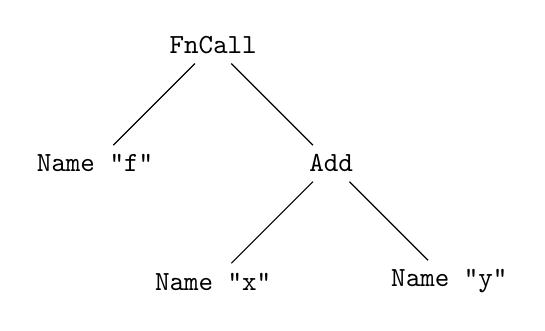
\begin{tikzpicture}[level distance=1.5cm,
    level 1/.style={sibling distance=3cm},
    level 2/.style={sibling distance=3cm}]
  \node{\texttt{FnCall}}
    child {node {\texttt{Name "f"}}}
    child {node {\texttt{Add}}
      child {node {\texttt{Name "x"}}}
      child {node {\texttt{Name "y"}}}
    };
\end{tikzpicture}
\end{center}

\vspace{0.5cm}

There are several different techniques of parsing, such as recursive descent and
LL. These methods often suffer from complex, unreadable code. However, Haskell's
type system allows me to use a different approach for parsing: parser
combinators. These allow you to use operators to combine simple parsers in
different ways to create complex ones. This technique of parsing is not without
issues - one of the main ones is that it is quite slow compared to conventional
techniques like recursive descent. However, the speed is still acceptable, and
their simplicity means that this is likely the technique I will use for parsing
my language.

\paragraph{Syntax inspiration}

The syntax of purely functional programming languages tends to be relatively
similar; they are mostly based off of either Haskell or Standard ML.
Haskell-like syntax looks like this:

\begin{verbatim}
  -- This is a comment
  foo :: Int -> Int  -- The type of "foo": it is a function from int to int
  foo x = x + 2      -- The definition of "foo": it adds 2 to its argument
\end{verbatim}

This is a very readable syntax, and has inspired other languages like OCaml.
However, it uses indentation for parsing; this can be quite complicated to do.
As such, for simplicity, I plan to change this syntax style slightly to allow
parsing without indentation. On the downside, this will make the syntax slightly
harder to read; however, it will simplify the parser greatly.

\paragraph{Language syntax}

My language's syntax will be approximately as follows:

\begin{verbatim}
  -- Line comments are started with two dashes

  {-
    Block comments are delimited like this
    {- They can also be nested -}
  -}

  -- Type signatures and bindings. The semicolon indicates the end of a
  -- top-level expression
  foo :: Int;
  foo = x;

  -- The following is the expression syntax.

  -- Function application (a function 'f' applied to a parameter 'x')
  f x

  -- Lambda abstractions (with a parameter 'x')
  λx -> e
  \x -> e

  -- let-bindings use semicolon-separated bindings enclosed in braces.
  -- The last binding may be terminated with an optional semicolon
  let { x = e0; y = e1 } in e2

  -- case expressions use semicolon-separated cases enclosed in braces.
  -- The last case may be terminated with an optional semicolon
  case { Cons x xs -> xs; Nil -> Nil }
\end{verbatim}

\subsubsection{Data types}

A more simple feature of Haskell is algebraic data types (ADTs). These are
datastructures which have multiple constructors, each containing some number of
values; for instance, a data type describing a list of integers could be
recursively defined in Haskell as follows:

\begin{verbatim}
  data IntList = Cons Int IntList | Nil
\end{verbatim}

This declaration specifies that an \verb'IntList' either consists of the
\verb'Cons' constructor applied to an \verb'Int' and another
\verb'IntList' (representing the rest of the list), or the \verb'Nil'
constructor applied to no arguments, which represents the empty list.
These constructors can be thought of as functions that just store their
arguments (and allow you to later extract them). This feature is shared
by non-lazy languages like OCaml and Standard ML; it allows for a
simple, intuitive, and safe representation of many data structures.

These types can also be polymorphic. For instance, the above
\verb'IntList' type can be generalised to any type as follows:

\begin{verbatim}
  data List a = Cons a (List a) | Nil
\end{verbatim}

\subsubsection{Type systems}

Another major feature of most functional languages is the type system.
Sophisticated type systems allow the programmer to specify very precise types
for values in the language; they act as a form of machine-checked documentation,
but also come with benefits like easy polymorphism.

Most ``interesting'' type systems are based on the lambda calculus, a theoretical
model for program execution (like Turing machines). There are three main type
systems to consider; the simply typed lambda calculus (hereafter referred to as
STLC for brevity), the Hindley-Milner type system, and System F.

\paragraph{Simply-typed lambda calculus}

STLC is, as the name suggests, effectively the most simple possible type
system for the lambda calculus. It allows polymorphic types to be
constructed using function arrows, written \verb'->', and named type
variables. For example, the term \verb'\x. x' could be ascribed the type
\verb'a -> a', representing a function from a value of some type
\verb'a' to that same type. Similarly, \verb'\f. \x. f x' could be
ascribed the more complex type \verb'(a -> b) -> a -> b', representing a
function which converts a function \verb'a -> b' and a value \verb'a'
into a value \verb'b'. This is an incredibly helpful theoretical model;
however, it is not so useful in practical programming languages, since
for both efficiency and ease of code we want many, many more types than
just functions. Additionally, the simply-typed lambda calculus is
Turing-incomplete, making it impractical for use in a programming
language.

\paragraph{Hindley-Milner typing}

The Hindley-Milner type system (sometimes referred to as Damas-Milner) extends
the STLC with the ability to work with types other than functions. This
is an incredibly popular type system for several reasons; the main one
is that type inference is completely decidable within this system.  This
means that given an expression with no type annotations (explicit pieces
of code informing the compiler of the type of expressions), the compiler
can always infer the most general (i.e.  polymorphic) type for an
expression by itself. This type system is used by the Haskell spec,
whose type system is effectively Hindley-Milner extended with
typeclasses. There also exists a relatively straightforward algorithm
for describing this type system, called Algorithm W. HM is proven to be
effectively as expressive as it is possible for a type system to be
whilst retaining decidability.

\paragraph{System F}

System F is a more sophisticated type system, implemented by modern GHC's
dialect of Haskell. It extends the Hindley-Milner system with rank N types - in
layman's terms, ``nested polymorphism''. For instance:

\begin{verbatim}
  \f. (f 3, f "hi")
\end{verbatim}

This is a lambda which applies a function, given as its argument, to the values
3 and ``hi''. Because these values have different types, this program cannot be
expressed in the Hindley-Milner type system. These more complex types can be
beneficial in several areas of code (hence GHC's support for them); however,
they also greatly increase the complexity of the type system. Type inference
within System F is undecidable; this means it requires user-supplied type
annotations for inference to be successful. There is also no standard algorithm
for type checking and inference of System F expressions; there are many
competing methods of doing this, such as bidirectional type systems (e.g. the
one described in ``Practical type inference for arbitrary-rank types''; S. Peyton
Jones, D. Vytiniotis, S. Weirich, M. Shields; Microsoft Research). Due to this
complexity, and the relatively few benefits, I will likely not implement the
System F type system in any capacity; instead, I plan to implement the
Hindley-Milner system.

\paragraph{Typeclasses}

Typeclasses are an extention to the Hindley-Milner (or System F) type system
which allow for increased polymorphism. An example of the motivation for these
is a sorting function; a comparison-based sorting function, under simple System
F, cannot be polymorphic. This is because it can not be applied to any type, but
rather only those which are ordered. Typeclasses are effectively a more powerful
version of interfaces as seen in OOP, and are Haskell's defining feature.
However, these complicate type inference and checking drastically, so while they
are a very helpful feature, they are not going to be a primary aim for this
project (although I may revisit them if I have time).

\subsubsection{Lazy evaluation}

Lazy evaluation is a feature of some programming languages where an
expression is not evaluated until its value is required. For instance,
in the following function:

\begin{verbatim}
  const :: a -> b -> a
  const x y = x
\end{verbatim}

The value of \verb'y' will never be evaluated when \verb'const' is
called. This means a call like the following...

\begin{verbatim}
  const 10 (factorial 100000000)
\end{verbatim}

...will not perform the expensive \verb'factorial' computation. This
language feature becomes useful in writing clean code. As an example, if
a program needs to generate an unkown amount of prime numbers, in an
imperative language you would have to write code which generated extra
ones as they were required. However, in a lazy language, you can simply
define an infinitely long list of prime numbers, and they will only be
computed as they are requested. This allows you to easily separate
production and consumption of data, making it easy to write clean code.

\begin{verbatim}
  -- A naive implementation of an infinite list of primes
  primes :: [Integer]
  primes = filter isPrime [2..]
\end{verbatim}

Laziness is a relatively broad term in programming langauges; languages like
Haskell provide purely lazy semantics, while some like OCaml allow you to opt-in
to laziness, and others like Perl 6 support laziness only in instances of
certain data structures (like lists). Here, we will be looking at a fully lazily
evaluated language, as in Haskell. This form of laziness can be incredibly
useful for defining recursive datastructures; for instance, the definition of an
infinite list in Haskell is simply as follows:

\begin{verbatim}
  x = 1 : x
\end{verbatim}

This definition works because the elements of x are only evaluated when they
need to be.

\paragraph{Bottom values}

To understand the basis for lazy evalution, we first need to discuss
bottom values.

In any sufficiently expressive (Turing-complete) language, you can write
non-total expressions: this means an expression that does not produce a
value. Examples of this include throwing exceptions, looping infinitely,
or recursing infinitely (by the undecidability of the Halting problem,
it is impossible to eliminate such programs computationally). We want to
be able to logically reason about these computations. As such, we say
that these non-terminating or erroring computations are represented by a
special value, ``bottom'', which we generally write as ⊥ or \verb'_|_'.
This value is incredibly special, as it is the only value which inhabits
all types (that is, ⊥ is a valid value of every type).

\begin{verbatim}
  f x = f (x + 1)  -- Calls to this function will never terminate
  f 3 = ⊥   -- Therefore, we can semantically say it returns ⊥
\end{verbatim}

\paragraph{Strict semantics}

Technically speaking, Haskell is not, by specification, a lazily
evaluated language; instead, it is non-strict. Non-strict means that
evaluation proceeds from the outside of an expression inwards, as
opposed to the other way round. The practical meaning of this is to do
with how bottom values propagate throughout expressions. In a strictly
evaluated language - such as most imperative languages - a bottom value
appearing in any subexpression will result in the entire expression
evaluating to bottom; for instance, a function call \verb'f(1, x)' would
neccesarily evalute to ⊥ if \verb'x' is ⊥. Non-strict
languages, on the other hand, could have \verb'f' return a perfectly
valid value. Strict languages often have a small amount of non-strict
behaviour in the form of boolean short-circuiting: in languages like C,
evaluating \verb'true || f(0)' will never call \verb'f', as it is not
neccesary to know that the entire statement returns \verb'true'.
Non-strict languages extend this to all aspects of the language's
syntax.

In practice, most, if not all, implementations of Haskell use laziness
as the method for implementing non-strictness. With lazy evaluation,
function application, rather than actually running code, creates a
datastructure called a ``thunk'', which describes the function and its
argument. Then, when this value is ``forced'' (its evaluation is
required), the function is actually called to calculate the result.

\paragraph{Evaluation}

In order to understand the implementation of laziness, we must first define what
``evaluation'' of an expression means. To do this, we define three ``forms'' of
expression; normal form (NF), head normal form (HNF), and weak head normal form
(WHNF).

\begin{itemize}

  \item An expression in normal form is effectively fully evaluated. More
  specifically, an expression in NF is either a data constructor applied to
  arguments all in NF, or a lambda abstraction whose body is also in NF.

  \item An expression in head normal form is either a data constructor applied to
  arguments (which may be in any form), or a lambda abstraction whose body is
  in head normal form.

  \item An expression in WHNF is either a data constructor applied to arguments
  (which may be in any form), or a lambda abstraction (whose body may be in
  any form).

\end{itemize}

The most important of these ``forms'' is weak head normal form (WHNF).
The way evaluation actually normally occurs in a lazy language is
through pattern matching, which effectively allows you to deconstruct a
type. For example, using the previously defined \verb'IntList':

\begin{verbatim}
  sum = \x -> case x of { Cons x xs -> x + sum xs; Nil -> 0 }
\end{verbatim}

This defines 'sum' as a lambda (anonymous function) of one argument
\verb'x'.  This argument (which should be an \verb'IntList') is then
deconstructed with a \verb'case' expression; this looks at the
constructor of x, and runs a different piece of code depending on the
constructor used. This case expression is the only way evaluation occurs
in most lazy languages. For this, we evaluate the expression (which may
be a thunk) into weak head normal form. This guarantees that, as long as
the value is of the correct type, the constructor in question will be
evaluated, and can be matched against.

\subsubsection{Garbage collection}

Like most high-level languages, this language will have automatic memory
management. Therefore, I will have to implement a garbage collector
(GC). There are several common types of garbage collector.

\paragraph{Reference counting}

Reference counting (refcounting) is one of the simplest methods of
garbage collection. In this method, every object managed by the GC has a
field in its header specifying how many other objects reference it (i.e.
have a pointer to it). Whenever another object makes a reference to this
object, its reference count is incremented. When a reference is deleted,
the reference count is decremented. After this decrement, it is also
checked whether the reference count has reached zero; if it has, the
object is freed.

This method of garbage collection has some advantages. One is that it
does not ``stop the world''; this means that, as oppose to most other
methods, the program never has to pause execution for an extended period
of time to allow the garbage collector to run. There is one exception to
this rule however, and it is one of the issues with refcounting;
occasionally, freeing one object can recursively remove many references
and free tens or hundreds of objects, resulting in a noticeable pause.
Refcounting is incredibly simple to implement. However, it has one more
major flaw: it fails to ever clean up any kind of recursive
datastructure. Due to immutability, this may not actually be a problem
in an eager purely functional language; however, lazy semantics allow us
to easily define recursive or mutually recursive datastructures. For
instance, a definition like \verb'x = 1 : x' defines an infinitely long
list of \verb'1's, and because it references itself (hence always has a
refcount of at least one), it would never be cleaned up, which could
result in a memory leak. For this reason, refcounting is rarely used as
a garbage collection method (at least, not in isolation).

\paragraph{Mark-and-sweep}

Mark-and-sweep garbage collectors are one of the most common designs for
GCs, used by languages such as Java and Go. In this design, at certain
times (generally when the heap reaches capacity), execution is paused
(this is a ``stop-the-world'' design), and garbage collection begins.
The garbage collector looks at all objects accessible from the current
scope of execution, and sets a special bit in the header to mark the
object as accessible. It then recursively does the same to all objects
referenced by these objects, and all objects referenced by those, etc.
It repeats this entire process for every stack frame and, at the end, it
has marked every ``active'' object (i.e. one which is accessible by
code). Finally, it iterates over all the allocated objects; any that are
not marked are freed.

This type of garbage collector does not have any issues with recursive
data structures; it will always be able to free as many objects as
possible. However, it can be quite slow; this can be seen in many larger
Java applications, which can have noticable pauses of around a second if
a lot of garbage is being created.

\paragraph{Generational}

A generational garbage collector allocates a small ``nursery'' of memory
where new allocations will occur, normally consisting of aroun 1MiB of
memory. Allocations occur sequentially in this nursery, until there is
not enough space remaining for a required allocation. At this point,
``minor GC'' is triggered. The garbage collector then does a
mark-and-sweep style check of all the objects on this nursery; it finds
those which are accessible by the program. However, instead of just
marking the objects as accessible, it copies them to a new
``generation'' on the heap (this makes it a ``copying GC'') and updates
all references to the object to the new pointer. Objects that are
inaccessible are not copied. After this process is complete, every
object in the nursery has either been found to be accessible, and copied
to the heap, or found to be inaccessible, and ignored. Therefore, no
object is stored in the nursery; so program execution can resume,
reusing the nursery for new allocations. Of course, occasionally, you
also need to perform garbage collection on the larger ``generation'';
this is called major GC. There are many variations on the basic design,
but the broad idea is to have separate regions of memory for different
ages of objects.

This can be a very powerful technique in purely functional languages.
This is due to immutability; because objects are immutable, it is
impossible for an object in a younger generation to be referred to by an
object in an older generation. This makes identifying referenced objects
faster and more efficient. As such, GHC generally employs a generational
approach to garbage collection. Recently, it has been updated to also
optionally use a more complex hybrid approach with mark-and-sweep which
can be more suitable for latency-sensitive programs. I will likely
implement a simple moving generational garbage collector, as it provides
a nice balance between efficiency and simplicity of implementation.

\subsubsection{Intermediate representations}

Compiling a high-level language like this to assembly is a complex task.
For this reason, compilers do not typically translate source directly;
instead, they move through one or more ``intermediate representations''
(IRs), each lower-level than the last. These are datastructures very
similar to an AST, with the difference that they do not correspond to
any literal source language. GHC uses three IRs: Core, STG and Cmm.

Core is GHC's first IR, and its most well-known. It is an incredibly
simple functional IR; similar to Haskell itself but much smaller.
Expressions in Core are defined as an ADT with the following 10
constructors:

\begin{verbatim}
  data Expr b    -- "b" for the type of binders
    = Var   Id
    | Lit   Literal
    | App   (Expr b) (Arg b)
    | Lam   b (Expr b)
    | Let   (Bind b) (Expr b)
    | Case  (Expr b) b Type [Alt b]
    | Cast  (Expr b) Coercion
    | Tick  (Tickish Id) (Expr b)
    | Type  Type
    | Coercion Coercion
\end{verbatim}

However, several parts of this type are not relevant - \verb'Tick'
relates to debugging information, and \verb'Coercion' and \verb'Cast'
are concerned with more complex features of GHC like functional
dependencies and type families. A simplified version of Core is as
follows:

\begin{verbatim}
  data Expr b    -- "b" for the type of binders
    = Var   Id
    | Lit   Literal
    | App   (Expr b) (Expr b)
    | Lam   b (Expr b)
    | Let   (Bind b) (Expr b)
    | Case  (Expr b) b Type [Alt b]
    | Type  Type
\end{verbatim}

This tells us that a Core expression is either a variable, a literal, a
function applied to an argument, a lambda abstraction, a set of let
bindings, a case expression, or a type. Types being in this IR seems
strange at first; the reason for this difference is that Core uses the
notion of type lambdas to represent polymorphism. A simple function like
\verb'id :: a -> a' is, in Core, represented as
\verb'id = \(@ t) -> \(x :: t) -> x', where the first parameter is the
type and the second is a value of that type. This facility is not
neccesary for HM-like type systems; it is only present in Core as this
language describes a variant of System F.  Also notice that Core
expressions are parameterized over a type \verb'b', describing bound
variables. This is used to add extra metadata to the IR.

I will likely use a Core-like IR in compilation of my language. This is
because it allows you to remove any syntactic sugar in the language, and
generally simplify the representation, before proceeding with
compilation. There will be two main differences between my IR and my
source language.

The first is in let bindings. Before or during type checking, let
bindings are split into ``binding groups''; groups of mutually recursive
bindings. Keeping this separation makes the IR slightly simpler to
compile later on.

The second is in case expressions. In the source language, pattern
matches may be nested arbitrarily:

\begin{verbatim}
  case xs of
    { Cons p (Cons q (Cons r Nil)) -> e0
    ; _ -> e1 } -- default case
\end{verbatim}

However, this cannot be directly compiled. Instead, the cases must be
flattened into matching single constructors:

\begin{verbatim}
  case xs of
    { Cons p tmp0 ->
      case tmp0 of
        { Cons q tmp1 ->
          case tmp1 of
            { Cons r tmp2 ->
              case tmp2 of
                { Nil -> e0
                ; _   -> e1 }
            ; _ -> e1 }
        ; _ -> e1 }
    ; _ -> e1 }
\end{verbatim}

For simplicity, my IR will require a default case in every pattern
match. If not provided in source, this will be automatically generated
as an expression that throws an error.

\subsection{Objectives}

\begin{itemize}

  \item Create a parser for a Haskell-like functional programming syntax into an AST

  \item Implement inference and checking for the Hindley-Milner type system with ADTs
  using Algorithm W

  \item Convert this AST into a simpler, untyped IR language

  \item Convert this IR into AMD64 assembly (which supports lazy evaluation with
    thunks), using a low-level runtime written in C

  \item Implement a garbage collector to prevent memory leaks in written code

\end{itemize}

\section{Design}

\subsection{High-level overview}

The compiler pipeline will have approximately the following stages:

\begin{itemize}
  \item CLI argument parsing: parse all the arguments given to the
    compiler, and set its state as specified.

  \item Code parsing: for each input file, parse the file's
    declarations into an AST, reporting errors if parsing fails.

  \item Type checking: Run the Algorithm W based type checker over each
    binding, reporting any type errors that occur.

  \item IR generation: Convert the AST to a simplified intermediate
    representation, flattening let bindings and performing other
    simplification steps.

  \item Code generation: Convert the IR into AMD64 assembly source.

  \item Assembly: Assemble the asm code into object files.

  \item Linking: Link all the compiled object files together alongside
    the runtime code.
\end{itemize}

Most of this functionality will be implemented in the compiler itself,
with two exceptions. Firstly, converting AMD64 assembly to machine code
is a complex process due to the highly complex and backwards-compatible
instruction encoding; therefore, I will use external utilities - likely
the \verb'nasm' assembler - to perform this stage. Secondly, linking
objects together is out of scope for this project, requiring in-depth
knowledge of the object format (ELF64 on Linux or PE on Windows) and
more. Therefore, I will also use external tools for this by calling into
the system linker \verb'ld'.

\subsection{CLI}

As with most compilers, my program will use a command-line interface.
The interface will take a series of flags followed by the names of the
files to compile; the specific usage will be defined by the following
manual page.

\begin{verbatim}

SYNOPSIS
  qntc [-S|-c] [-v] [-static|-shared] [-On] [-o outfile] infile...

DESCRIPTION
  qntc reads the quanta source files specified by 'infile' and compiles them
  into a binary specified by 'outfile'.

  By default, qntc will compile the files specified on the command-line by
  'infile' to an executable. This executable will be named as specified by
  'outfile' or, if 'outfile' is not specified, a default name based on the
  platform ('a.out' on Linux; 'out.exe' on Windows).

  Flags '-S' and '-c' change the type of file the compiler outputs.  Normally,
  the compiler performs compilation, assembly, and linking; however, if given
  '-S', the compiler will not assemble, and if given '-c', the compiler will
  assemble each file, but will not link them together.

  qntc uses 'nasm' and 'ld' internally for compiling asm to object files and
  linking object files into binaries. If 'nasm' is not in PATH, and '-S' is not
  given, qntc will return an error. If 'ld' is not in PATH, and neither '-S' nor
  '-c' is given, qntc will return an error.

OPTIONS
  -S          Compile, but do not assemble; output asm files. The created files
              will be in amd64 NASM syntax. If 'outfile' is not specified and
              there are multiple input files, the output filenames are the input
              filenames with '.asm' concatenated on the end. If 'outfile' is
              specified and there are multiple input files, the output filenames
              are the input filenames with '.outfile' concatenated on the end.
              If 'outfile' is not specified and there is a single input file,
              the output file is 'out.asm'. If 'outfile' is specified and there
              is a single output file, the output filename is 'outfile'.

  -c          Compile and assemble, but do not link; output object files. This
              is subject to the same naming rules as '-S', except the '.o' file
              extension is used in place of '.asm'.

  -v          Enables verbose mode. In this mode, the compiler will output
              timestamped information about every stage of compilation. This
              exists primarily for compiler debugging, but may be useful
              elsewhere.

  -static     (default) Enables the use of static linkage for the produced
              binary. This has no effect if '-S' or '-c' is given.

  -shared     Enables the use of shared (dynamic) linkage for the produced
              binary. This has no effect if '-S' or '-c' is given.

  -On         Set the optimisation level to 'n'. 'n' may be any integer from 0
              to 9 inclusive; it specifies how aggressively optimisations should
              be performed, where 0 means "perform no optimisations" and 9 means
              "perform all optimisations". Note that higher optimisation levels
              are not guaranteed to have any effect.

  -o outfile  Set the output filename.

\end{verbatim}

\subsection{Algorithm W}

Algorithm W is a relatively simple algorithm for Hindley-Milner type
inference/checking. It was the original algorithm used for
Hindley-Milner type inference - described by Milner in 1978 - and has
stood the test of time as being relatively easy to implement whilst also
efficient enough for reasonable use.

An implementation of the HM type system has three important data types:
\verb'Type', \verb'TypeScheme' and \verb'Kind'. Types are the types
we're familiar with; they contain some type names, possibly with
application for polymorphic types like \verb'List'. However, this raises
an important point: we need to disallow objects with types like
\verb'List', as these are type constructors, not inhabited types. The
logic to this system is described by the ``kind'' of a type. Kinds are
effectively types of types; the kind \verb'*', or \verb'Star', is the
kind of an inhabited type (one that can have values, e.g. \verb'Int' and
\verb'List String'), and kinds can also be made with an arrow - i.e.
\verb'a -> b' is the kind of a type which takes a type argument of kind
\verb'a' and gives back a type of kind \verb'b'. The ability of a type
to have kinds other than \verb'Star' is referred to as ``higher-kinded
types''; this is an important feature of most functional languages.
Lastly, a type scheme is a description of a polymorphic type; it is a
type alongside a list for universally quantified (i.e. polymorphic) type
variables. These data types are defined in Haskell as follows:

\begin{verbatim}

  data Type
    = TConc Text   -- Conc meaning 'concrete' - i.e. a specific type
    | TVar Integer
    | TApp Type Type

  data TypeScheme
    = TypeScheme (Set Integer) Type

  data Kind
    = KStar
    | KArrow Kind Kind

\end{verbatim}

My definition of \verb'Type' will be slightly different to this. As I
want to support user-supplied type signatures with arbitrary names for
polymorphic variables, I plan to make \verb'TVar' store a \verb'Text',
and add another constructor \verb'TUnif' for unification variables (the
formal name for type variables used during type checking / inference):

\begin{verbatim}

  data Type
    = TConc Text
    | TVar Text
    | TUnif Integer
    | TApp Type Type

\end{verbatim}

Note that as a function type \verb'a -> b' is merely syntactic sugar for
\verb'(->) a b', functions \verb'a -> b' are represented as
\verb'TApp (TApp (TConc "->") a) b'.

Algorithm W works by generating unification variables to stand for
unknown types, and, as values are used in contexts that limit their
type, generating a ``substitution'' - via a process called
``unification'' - which describes more specific ways of representing a
unification variable. It can be described using a set of type rules.

\subsubsection{Typing rules}

TODO

\subsection{Runtime}

I have previously mentioned the language's runtime. This will be a piece
of code written in C (and potentially some assembly) which contains its
initialization code and garbage collector, as well as any other common
routines that turn out to be neccesary in compiled code. This will be
stored in either an object file or a static library file, and
automatically linked against the generated objects by the compiler.

\subsection{In-memory object representation}

An important consideration for a compiled language is how objects will
be represented in-memory at runtime. One of the advantages of static
type checking is that unlike languages like Python, all type information
can be erased at runtime; this slightly decreases memory usage, and
speeds up the code as types do not have to be checked during execution.

An object (closure) can be modelled as a header, followed by some number
of 1-word (8-byte) values, some of which are pointers. The header
contains three main things. The first is a number describing the type of
the object. This does not refer to the type in the context of the source
language, but rather whether the object represents a thunk, a data
constructor, or a function. The second thing the header contains is a
record of how long the object's body is (how many 64-bit values are in
it). This, combined with the object type, tells the garbage collector
(GC) everything it needs to know about the object; specifically, how
long the body is, and which fields are pointers to other objects.

There are a few more types of object in memory. One is an indirection.
When a thunk is evaluated, we want to update it in memory to contain the
value it was evaluated to. However, this raises an issue: thunks are
only large enough to hold two pointers in their closure, but the
evaluated value may require many more. For this reason, instead of being
directly replaced by the value, the thunk is replaced with an
indirection. This is an object which simply refers to another; it
contains no extra information.  As an optimisation, the garbage
collector could clean up these indirections by replacing references to
them with references to their target object.

The last two object types are to do with global values. Initially,
global values are essentially represented by a small piece of code
which, when run, will evaluate the object. This type of object can be
represented by a pointer to code. After the object is evaluated, the
global replaced with an indirection to the evaluated object. However, if
a normal indirection was used, the garbage collector would attempt to
clean up global indirections, which will cause errors; therefore, the
last object type is a so-called ``global indirection'', which acts
identically to a regular indirection except it will not be garbage
collected.

\begin{itemize}
  \item For thunks, the body simply contains two pointers: a pointer to
    the function object to be called, and a pointer to the object which
    is its argument.

  \item For ADT instances, the body contains a non-pointer encoding
    which constructor was used, and some number of pointers referencing
    the ADT's parameters.

  \item For primitive data types (e.g. \verb'Nat'), the body simply
    contains a non-pointer encoding the value. These primitives can be
    thought of as ADTs with a very large number of constructors and no
    extra parameters.

  \item For functions, the body contains a pointer to the entry code,
    followed by some number (possibly zero) of pointers to values
    referenced by the function's closure.

  \item For indirections (global or otherwise), the body contains a
    single pointer to the referenced object.

  \item For unevaluated global objects
\end{itemize}

This object layout can be understand as the following set of C
declarations, assuming packed structs and 64-bit pointers:

\begin{verbatim}
  #define OBJ_FUN   0
  #define OBJ_DATA  1
  #define OBJ_THUNK 2
  #define OBJ_IND   3
  #define OBJ_GLOBL 4
  #define OBJ_GLOBL_IND 5

  struct obj_header {
    uint32_t obj_type;
    uint32_t body_len;  // Total number of 64-bit values allocated in the body
  };

  struct object {
    struct obj_header hdr;

    union {
      struct {
        struct object *(*code)(struct object *arg, struct object *fun);
        struct object *closure_objs[];
      } fun;

      struct {
        uint64_t constr_id;
        struct object *closure_objs[];
      } data;

      struct {
        struct object *func;
        struct object *arg;
      } thunk;

      struct {
        struct object *target;
      } ind;

      struct {
        struct object *(*code)(void);
      } globl;
    };
  };
\end{verbatim}

\section{Technical Solution}

Before I begun the main implementation, I decided to define some
datatypes which would be important later. Firstly, I defined a small
collection of types as follows.

\begin{verbatim}
newtype Module = Module [Text]
  deriving (Show, Ord, Eq)

data Qual = Qual Module Text
  deriving (Ord, Eq)

data RName
  = QualName Qual
  | LoclName LName
  deriving (Ord, Eq)

data LName
  = SrcName Text
  | GenName Text
  deriving (Ord, Eq)
\end{verbatim}

The \verb'Module' datatype is simply a wrapper around a list of strings
describing a module name; for instance, the module \verb'Data.Nat' is
encoded as \verb'Module ["Data","Nat"]'. \verb'Qual' refers to a
fully-qualified name; it is simply a module alongside another string
(the name of the entity being referred to, for instance the \verb'add'
in \verb'Data.Nat.add'). \verb'LName' describes a name from a local
definition, for instance in a \verb'let' expression. It has two
constructors; \verb'SrcName', describing a name which appeared in the
original source code, and \verb'GenName', describing a name which has
been generated by the compilation process (these appear, for example, in
the unrolling of pattern matches). \verb'GenName' could be considered
unneccesary; however, it provides a very simple way to prevent name
conflicts between the original source and generated code. Lastly,
\verb'RName' is a resolved name; it can either be a fully-qualified
name, or some local name.

Next, I decided to define the data types describing the language's AST
in the module \verb'QntSyn' (Quanta syntax). This file ended up being
relatively complex. This is because as the compilation advances, the AST
should be annotated with additional information; for instance, after the
source is parsed, references to names should be resolved to the
locations they reference, turning simple references like \verb'add' into
resolved references like \verb'Data.Nat.add' (where \verb'Data.Nat' is
the module the \verb'add' function is defined in). It is possible to
perform this stage during code generation; however, separating it into a
separate stage making debugging easier later, and makes the code
clearer. Other information that must be annotated includes type
information, added by the typechecker. This information is not strictly
neccessary in compilation for a simple language like this; however, it
may be neccessary for more complex extensions such as typeclasses, and
it can again make debugging the compiler easier.

I modelled this ability to annotate the type using several features of
GHC's variant of Haskell. First, I created a simple enum datatype
\verb'TqcPass', describing the current stage of compilation.

\begin{verbatim}
data TqcPass
	= Parsed
	| Renamed
	| Typechecked
\end{verbatim}

Using the \verb'DataKinds' extension, I was able to parameterise the AST
types over the current pass. In order to change the structure of the AST
depending on this parameter, I used another GHC extension:
\verb'TypeFamilies'. This allowed me to scrutinise the pass given and
use different types for components of the AST based upon it. For
example, a type family named \verb'Id' was created to represent the type
of an identifier in a given pass. In the \verb'Parsed' stage, an
identifier is simply represented by a string. However, in the
\verb'Renamed' and \verb'Typechecked' stage, it is instead represented
by a different type that refers to either a local name or a
fully-qualified name. This type family is defined as follows.

\begin{verbatim}
type family Id p where
  Id 'Parsed = Text
  Id 'Renamed = RName
  Id 'Typechecked = RName
\end{verbatim}

Lastly, I needed to define one more helper type. A vital aspect of a
compiler is its error reporting, and an important component of error
reporting is accurately reporting the location of the code causing the
error. As such, my AST had to be annotated with location information
periodically so that error reporting could be accurate. I did this
through the definition of some more simple datatypes.

\begin{verbatim}
data SrcSpan = SrcSpan SourcePos SourcePos
  deriving (Show, Eq)

instance Semigroup SrcSpan where
  SrcSpan s0 e0 <> SrcSpan s1 e1 = SrcSpan (min s0 s1) (max e0 e1)

data Located a = L SrcSpan a
  deriving (Functor, Foldable, Traversable)

unLoc :: Located a -> a
unLoc (L _ x) = x
\end{verbatim}

The first type, \verb'SrcSpan', simply describes an area in source code.
It is defined by two source positions, and it has a way of combining
them; combining two spans simply creates a new span that encompasses
both of them. The second datatype, \verb'Located', associates a value of
an arbitrary type with a \verb'SrcSpan'. This allows us to easily
annotate source positions by, for instance, replacing an \verb'Expr'
with a \verb'Located Expr'. Because prefixing \verb'Located' can
sometimes be repetitive, I adopted the convention of defining type
aliases prefixed with an L to represent a located variant of a type; for
instance, \verb'LExpr Typechecked' is equivalent to
\verb'Located (Expr Typechecked)'.

With this and some similar type families defined, I next defined the AST
itself. The surface syntax of Quanta is relatively complex; as such,
this file contains a relatively large collection of mutually recursive
datatypes. The most important of these is the \verb'QntExpr' type,
describing the syntax of an expression. It is defined as follows:

\begin{verbatim}
data QntExpr p
  = QntVar (Id p)
  | QntNatLit Natural
  | QntApp (LQntExpr p) (LQntExpr p)
  | QntLam (Binder p) (LQntExpr p)
  | QntLet [QntBind p] (LQntExpr p)
  | QntCase (LQntExpr p) [LQntAlt p]
\end{verbatim}

This type encodes every form of expression in the language:
\begin{itemize}
	\item A variable reference (i.e. a name)
	\item A numeric literal
	\item An application of two expressions
	\item A lambda abstraction, containing a variable binder and a body expression
	\item A let expression, containing a list of binds and a body expression
	\item A case expression, containing an expression (the scrutineee) and a list of alternatives
\end{itemize}

This expression type uses the following ``utility'' types:

\begin{verbatim}
data QntBind p
  = QntImpl (Binder p) (LQntExpr p)
  | QntExpl (Binder p) (LQntExpr p) (LScheme (TyId p))

data QntPat p
  = QntNamePat (Binder p)
  | QntNatLitPat Natural
  | QntConstrPat (Constr p) [QntPat p]

data QntAlt p = QntAlt (QntPat p) (LQntExpr p)
\end{verbatim}

\end{document}
